\chapter{Phase 3 - Bonding to LEDs}
\label{sec:BondingToLEDS}
\section{Process}
In this section functional LEDs will be used to test the entire process and validate that this process can then later be used to bond a BP with actual transistors. The most major difference between this experiment and the previous ones will be the fact that the LEDs will consist of a `mesa' structure. This structure will require that the electroplating process can complete conformal coating onto the structure.

The GDS files for the LED, BP and overlay of both are in figure \ref{fig:P3_GDS_All}.

\begin{figure}
    \centering
    \begin{subfigure}[t]{0.3\textwidth}
        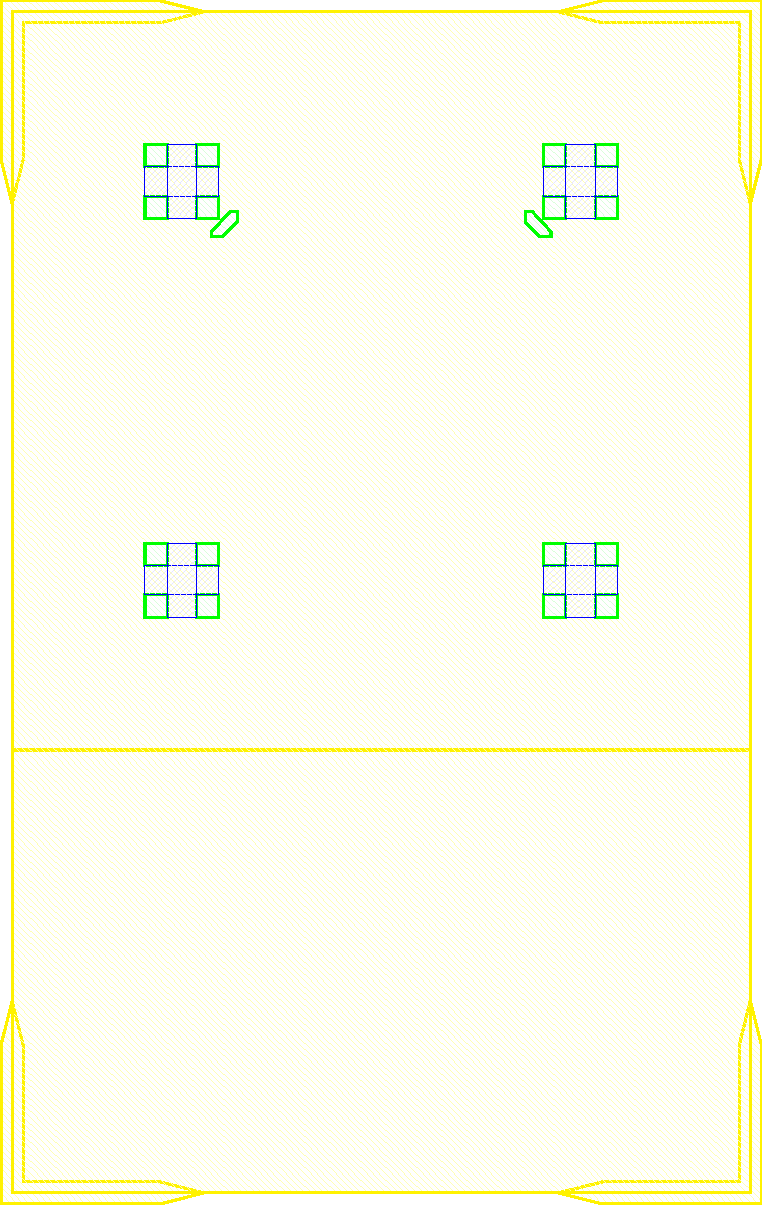
\includegraphics[width=\textwidth]{Main/Ch4/ONOFF_NC_2022_V3.GDS_BP.pdf}
        \caption{GDS file of BP.}
        \label{fig:P3_GDS_BP}
    \end{subfigure}
    ~
    \begin{subfigure}[t]{0.3\textwidth}
        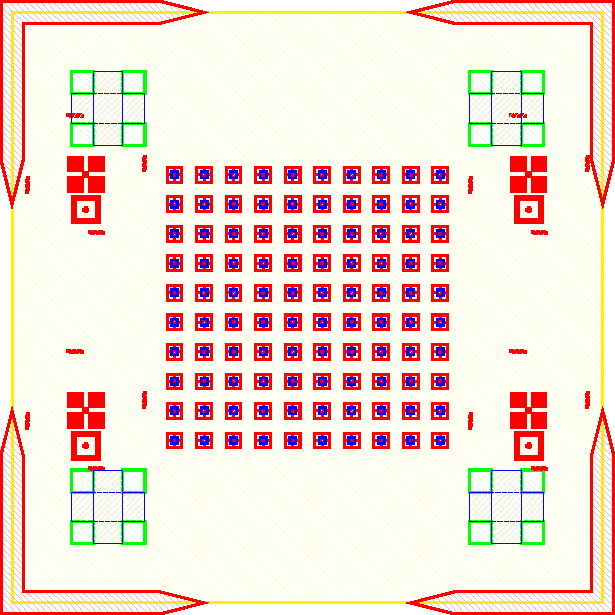
\includegraphics[width=\textwidth]{Main/Ch4/ONOFF_NC_2022_V3.GDS_LED.pdf}
        \caption{GDS file of LED.}
        \label{fig:P3_GDS_LED}
    \end{subfigure}
    ~
    \begin{subfigure}[t]{0.3\textwidth}
        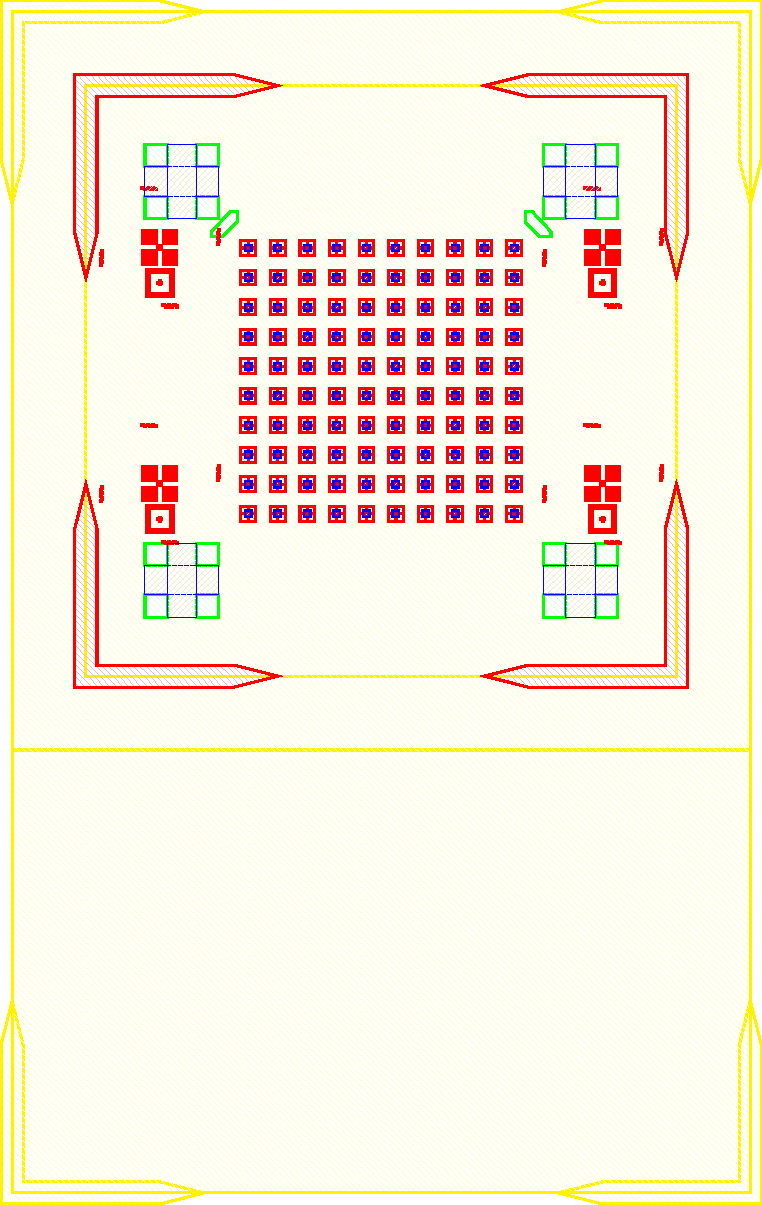
\includegraphics[width=\textwidth]{Main/Ch4/ONOFF_NC_2022_V3.GDS_BOTH.pdf}
        \caption{GDS file of overlay of LED on BP.}
        \label{fig:P3_GDS_BOTH}
    \end{subfigure}
    \caption{GDS files of Phase 3 samples.}
    \label{fig:P3_GDS_All}
\end{figure}

\section{Bonding Issues}

Upon attempting to diebond the LED to the backplane, all 3 attempts failed, the remaining BP and LED were withheld to do SEM imaging. From the images taken, it appeared to be that the bonds had a very insufficient thickness of indium present. However, the coating of indium did appear to be conformal.

As seen from the SEM images of the non-bonded samples in figures \ref{fig:P3_non_bonded_LED} and \ref{fig:P3_non_bonded_BP} the thickness of indium that was generated during the electroplating process was not nearly thick enough for the expected results of $4-6\um$. I believe that this was likely an issue that arose due to the poor formation of electric fields during the electroplating process as most other variables were fairly well accounted for.


\begin{figure}
    \centering
    \begin{subfigure}[t]{0.45\textwidth}
        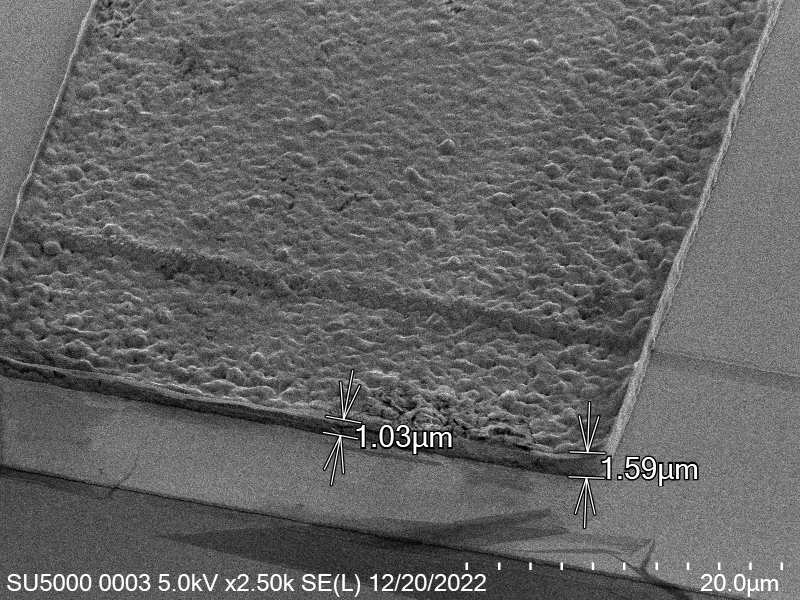
\includegraphics[width=\textwidth]{Main/Ch4/Phase-4/Non-Bonded/LED/IMG_No0003.png}
        \caption{Non-bonded SEM image of LED}
        \label{fig:P3_non_bonded_LED}
    \end{subfigure}
    ~
    \begin{subfigure}[t]{0.45\textwidth}
        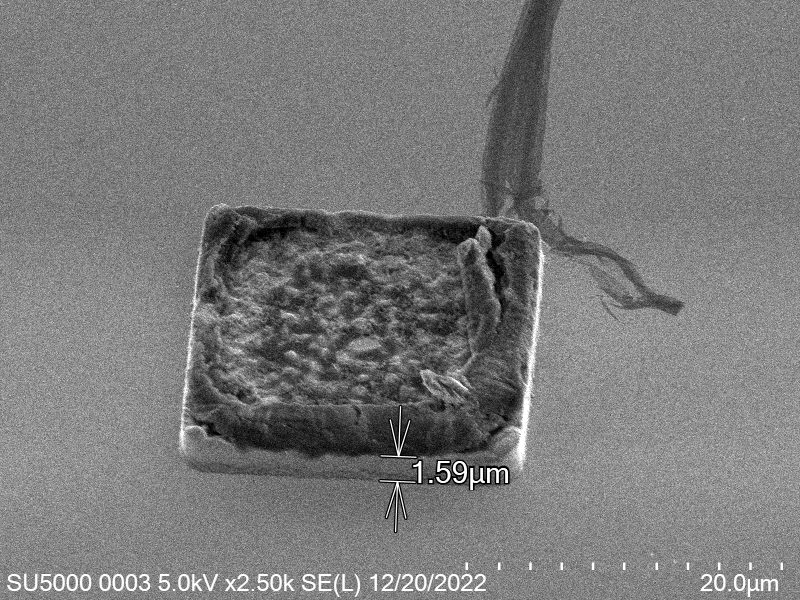
\includegraphics[width=\textwidth]{Main/Ch4/Phase-4/Non-Bonded/BP/IMG_No0003.png}
        \caption{Non-bonded SEM image of BP}
        \label{fig:P3_non_bonded_BP}
    \end{subfigure}
    ~
    \begin{subfigure}[c]{0.45\textwidth}
        \centering
            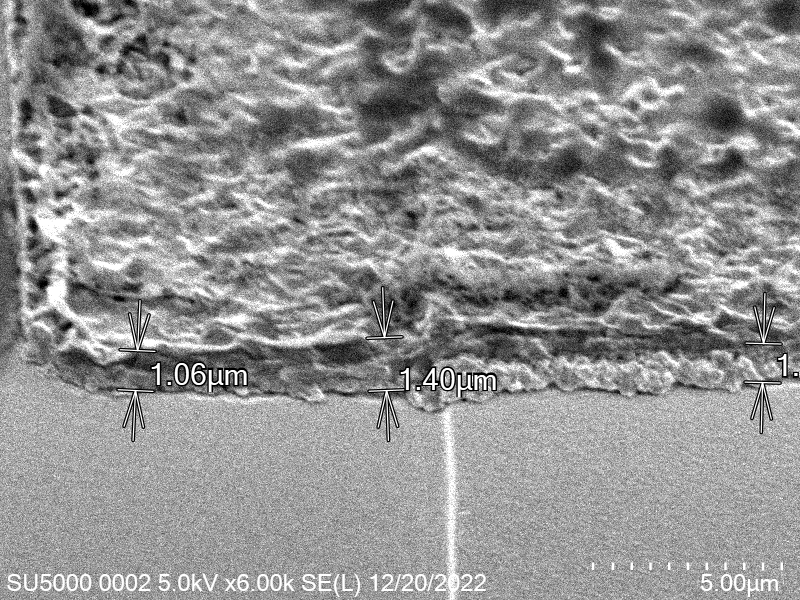
\includegraphics[width=0.48\textwidth]{Main/Ch4/Phase-4/P4-T02/LED/IMG_No0002.png}
            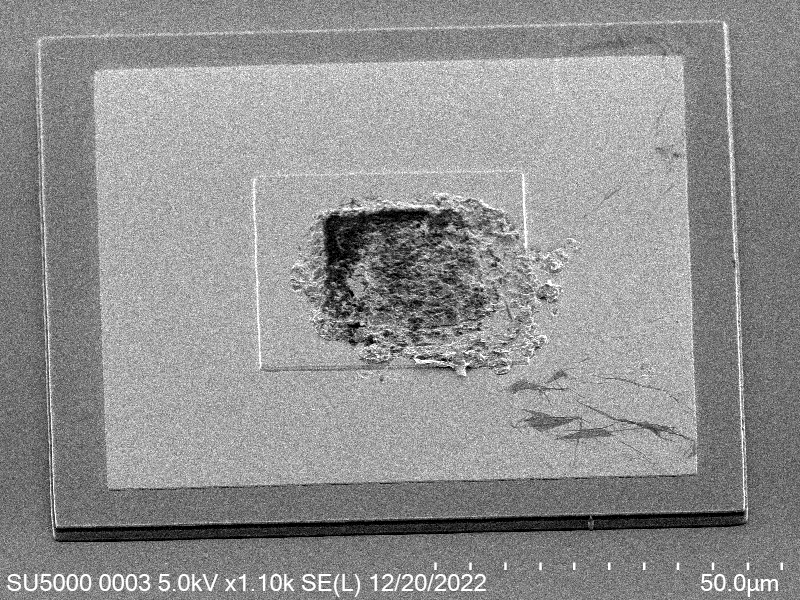
\includegraphics[width=0.48\textwidth]{Main/Ch4/Phase-4/P4-T02/LED/IMG_No0003.png} \\
            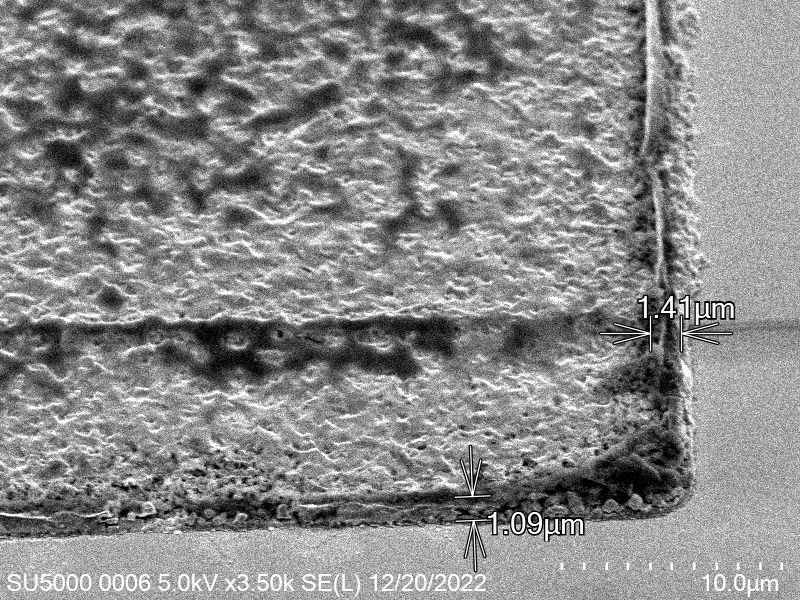
\includegraphics[width=0.48\textwidth]{Main/Ch4/Phase-4/P4-T02/LED/IMG_No0006.png}
            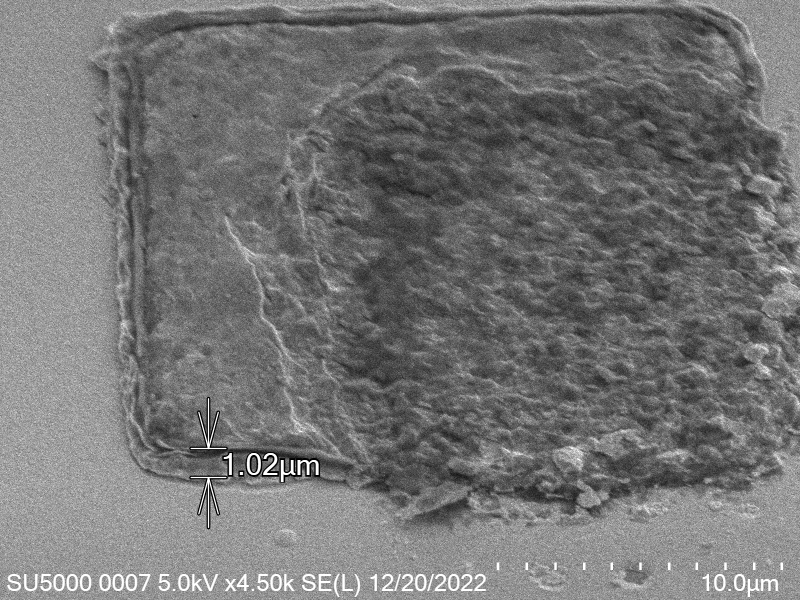
\includegraphics[width=0.48\textwidth]{Main/Ch4/Phase-4/P4-T02/LED/IMG_No0007.png}
        \caption{Bonded SEM images of LED}
        \label{fig:P3_bonded_LED}
    \end{subfigure}
    ~
    \begin{subfigure}[c]{0.45\textwidth}
        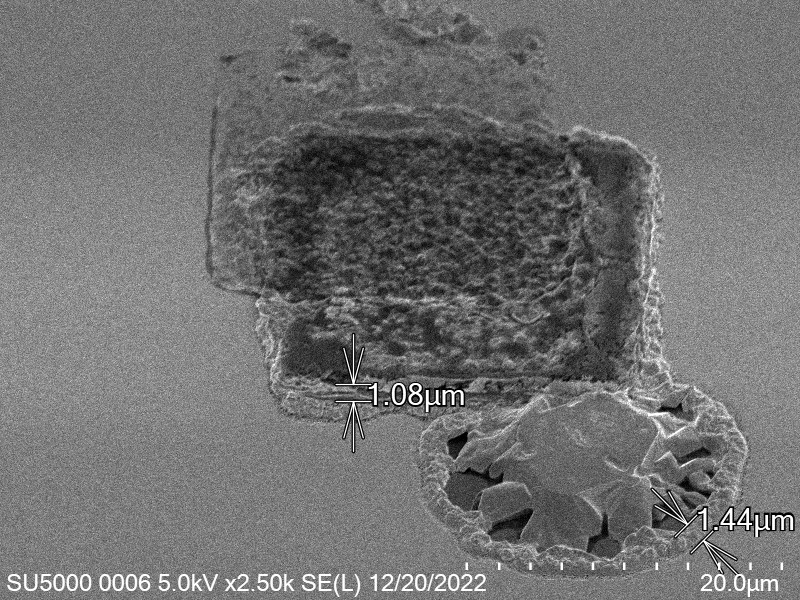
\includegraphics[width=\textwidth]{Main/Ch4/Phase-4/P4-T02/BP/IMG_No0006.png}
        \caption{Bonded SEM image of BP}
        \label{fig:P3_bonded_BP}
    \end{subfigure}
    \caption{SEM images of non-bonded (\ref{fig:P3_non_bonded_LED}, \ref{fig:P3_non_bonded_BP}) and bonded (\ref{fig:P3_bonded_LED}, \ref{fig:P3_bonded_BP}) LED BP pairs.}
    \label{fig:P3_SEM_All}
\end{figure}

To analyze this further, 2D electrical simulations were conducted to understand how the electric fields are generated during the electroplating process. The reference code can be seen in Appendix \ref{sec:Efield}.

The resulting electric field from the code looks like figure \ref{fig:field_lines}.



\begin{figure}
    \centering
    \begin{subfigure}[t]{0.45\textwidth}
        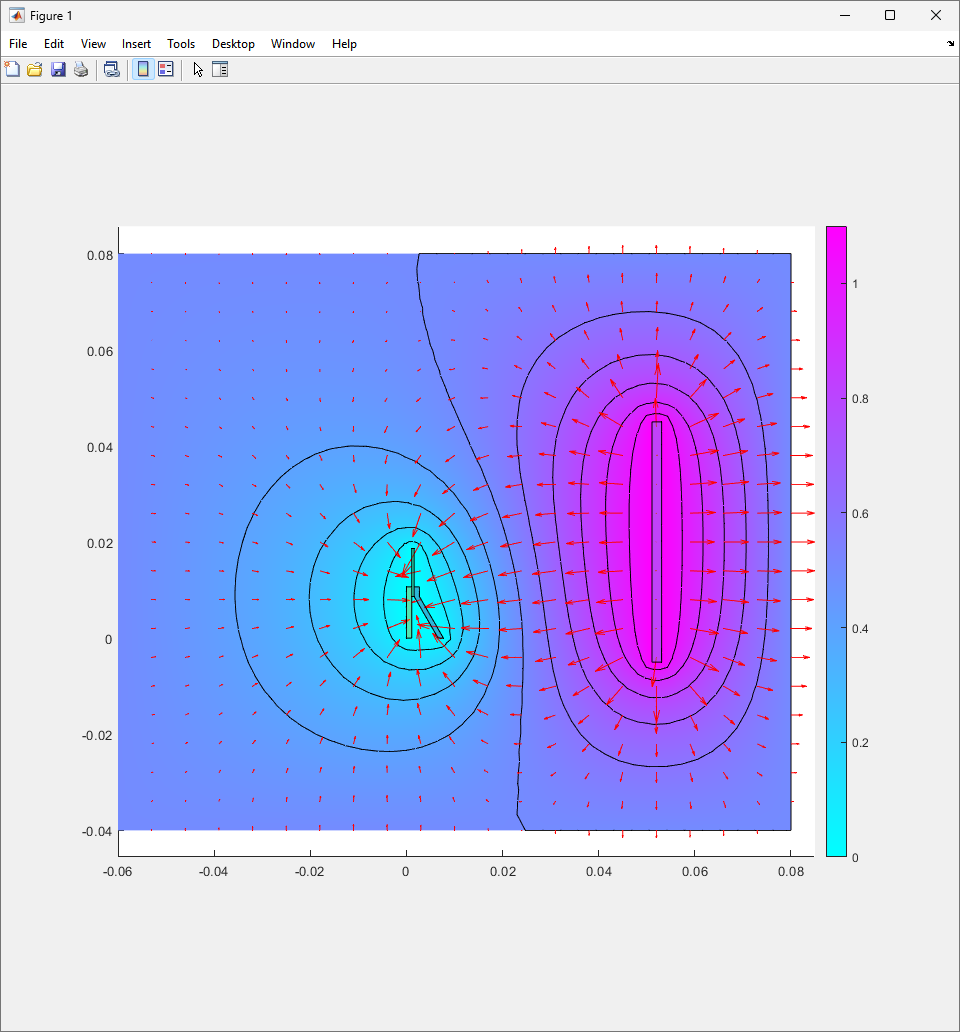
\includegraphics[width=\textwidth]{Main/Ch4/dirty_field_lines_aligator.png}
        \caption{Dirty electric field lines as a result of the alligator clip in solution.}
    \end{subfigure}
    ~
    \begin{subfigure}[t]{0.45\textwidth}
        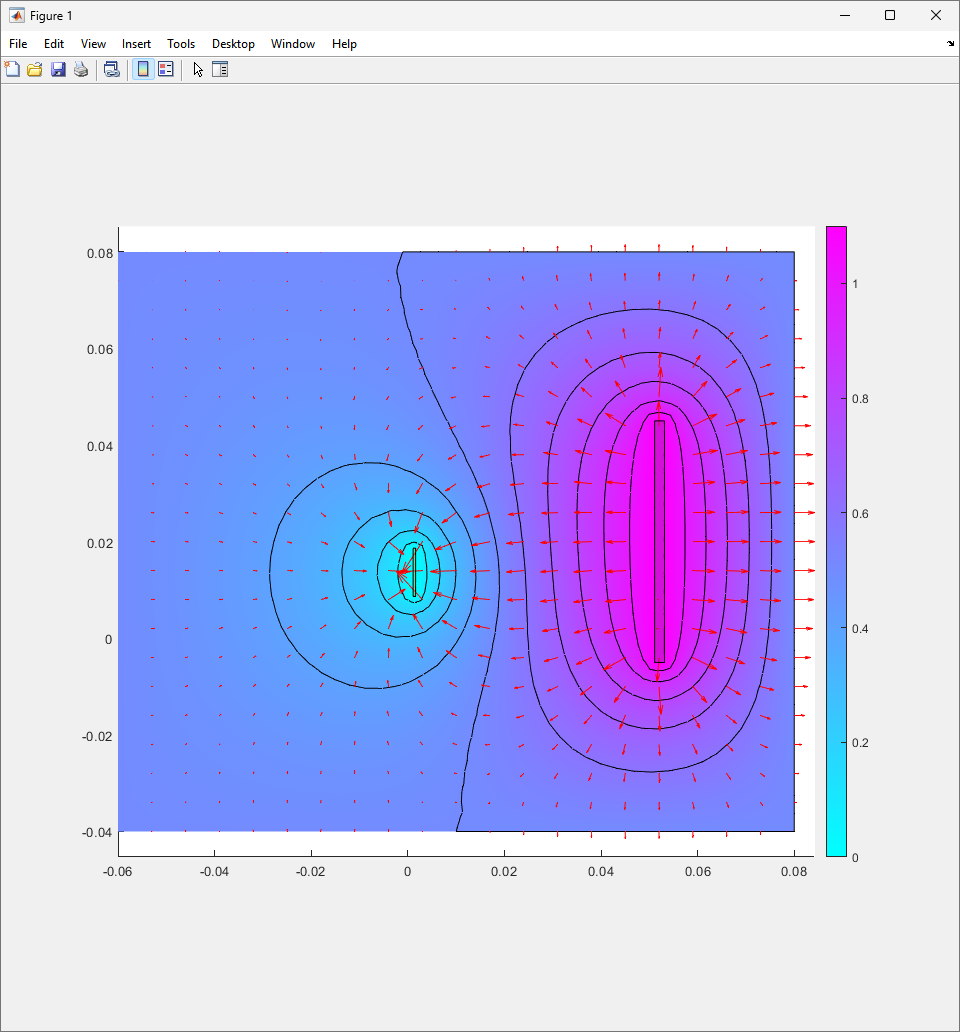
\includegraphics[width=\textwidth]{Main/Ch4/clean_field_lines.png}
        \caption{Clean electric field lines when there would be no alligator clip present.}
    \end{subfigure}
    \label{fig:field_lines}
\end{figure}


\section{Conformation to Theory}
As the theory from the previous section would suggest that there would be a greater flux of indium into the sections near the alligator clip. This can be clearly seen in figure \ref{fig:bumpVolumeMap} where there is a significant bias of indium near the region with the alligator clip attached.

The


\section{Development of a Repeatable Process}

The existing process failed after verification of previous metrics. As many of the previous issues were resolved methodically, there is likely an inherent flaw with the existing electroplating setup.

To improve the electroplating process I would like to complete the following goals:

\begin{itemize}
    \item Minimize movement of overall system.
    \item Make electric field lines more uniform.
    \item Minimize variability between electroplating runs.
\end{itemize}

To achieve the previous goals, I would like to propose the following solutions:

\begin{itemize}
    \item Fix the anode(indium bar) into a rigid fixture that maximizes flatness of the bar.
    \item Fix the distance between the anode and cathode with a rigid structure.
    \item Maximize uniformity of the electric fields by ensuring no other conductors are available on the same plane or between the anode and cathode.
\end{itemize}

To complete these goals a number of 3D models were designed and revised until they could meet the design requirements.

Furthermore, once the designs have been prototyped, it is necessary that appropriate materials are selected to function appropriately in the chemical conditions that the sample experiences.


\begin{figure}
    \centering
    \begin{subfigure}[t]{0.8\textwidth}
        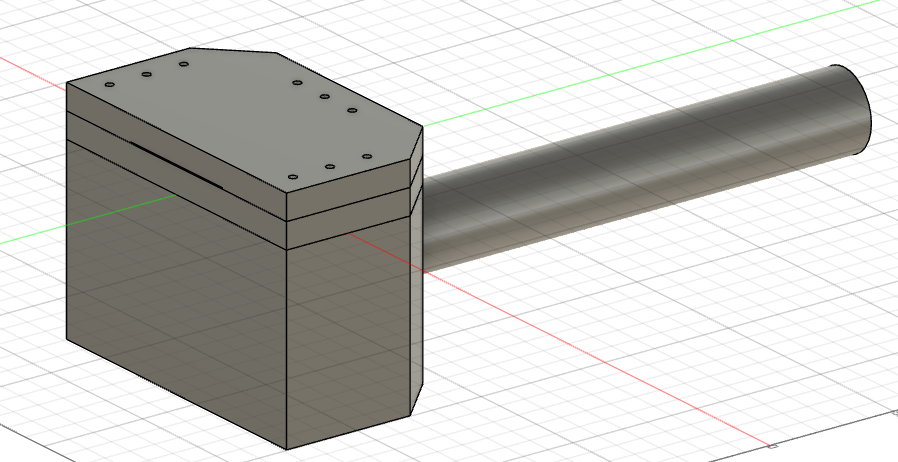
\includegraphics[width=\textwidth]{Main/Ch4/3D_models/clamp-overall.png}
        \caption{Overall 3D model of assembly.}
    \end{subfigure}
    ~
    \begin{subfigure}[t]{0.3\textwidth}
        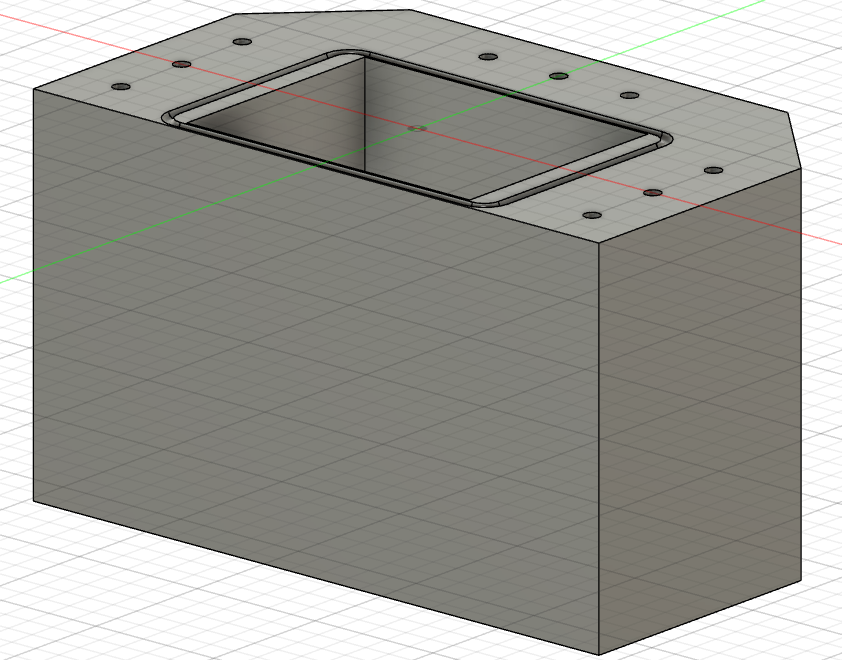
\includegraphics[width=\textwidth]{Main/Ch4/3D_models/clamp-bottom-top.png}
        \caption{Clamp back-section top view.}
        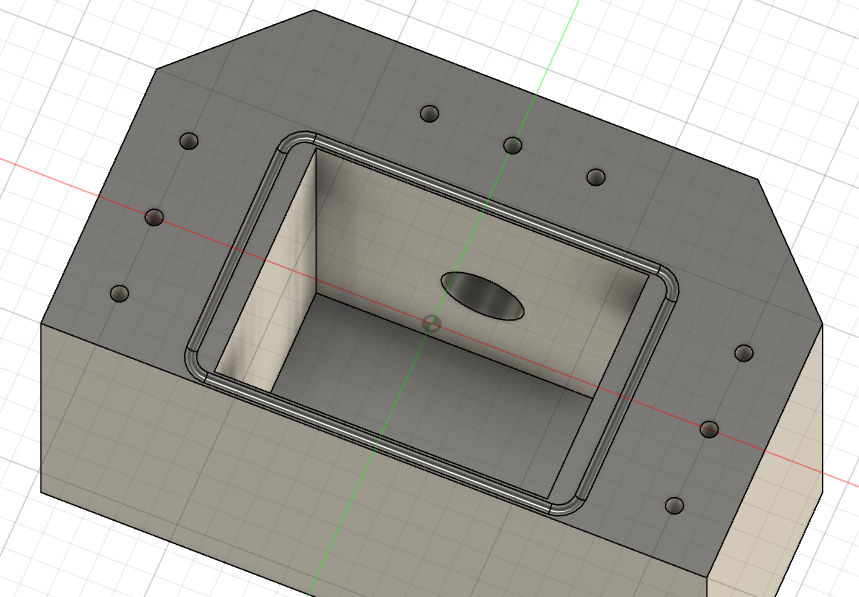
\includegraphics[width=\textwidth]{Main/Ch4/3D_models/clamp-bottom-top-2.png}
        \caption{Clamp back-section alternate view.}
    \end{subfigure}
    ~
    \begin{subfigure}[t]{0.3\textwidth}
        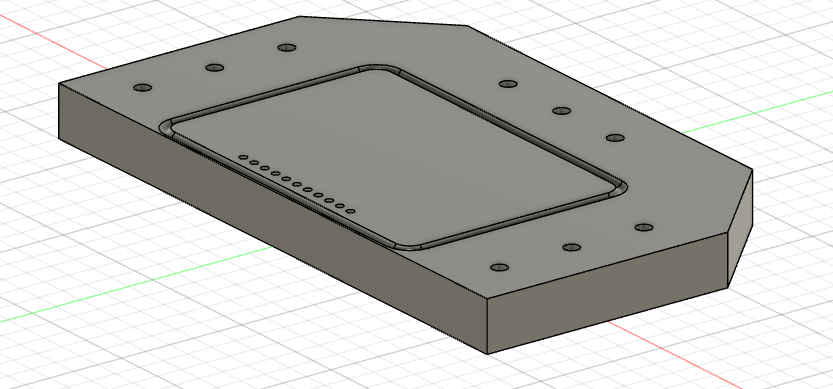
\includegraphics[width=\textwidth]{Main/Ch4/3D_models/clamp-middle-top.png}
        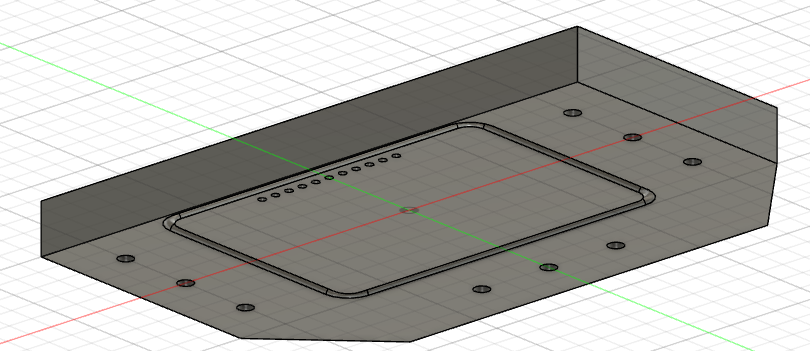
\includegraphics[width=\textwidth]{Main/Ch4/3D_models/clamp-middle-bottom.png}
        \caption{Clamp middle-section, part is symmetric.}
    \end{subfigure}
    ~
    \begin{subfigure}[t]{0.3\textwidth}
        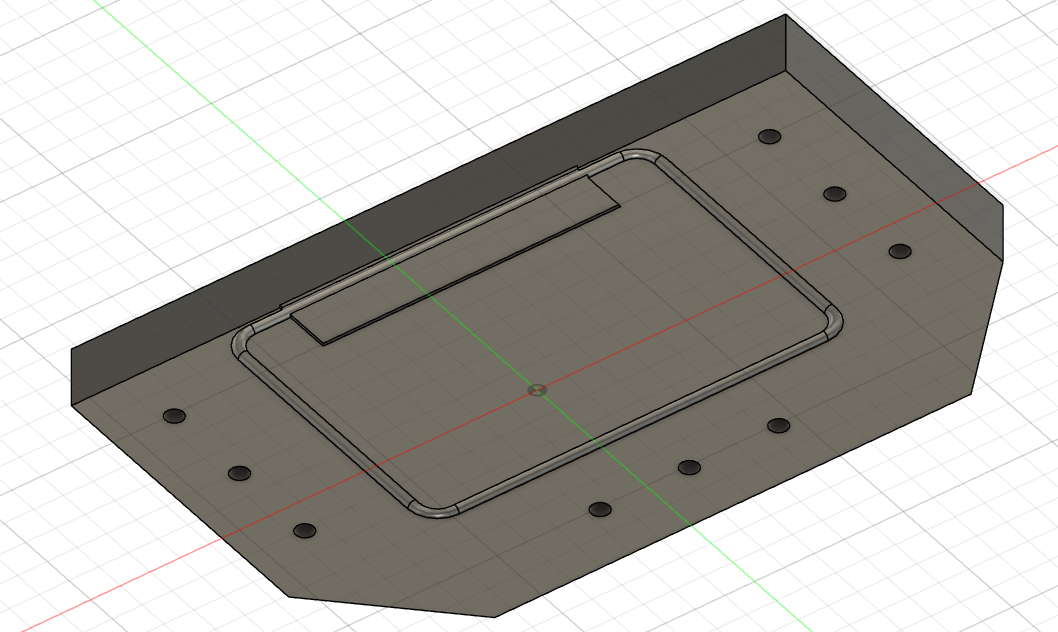
\includegraphics[width=\textwidth]{Main/Ch4/3D_models/clamp-top-bottom.png}
        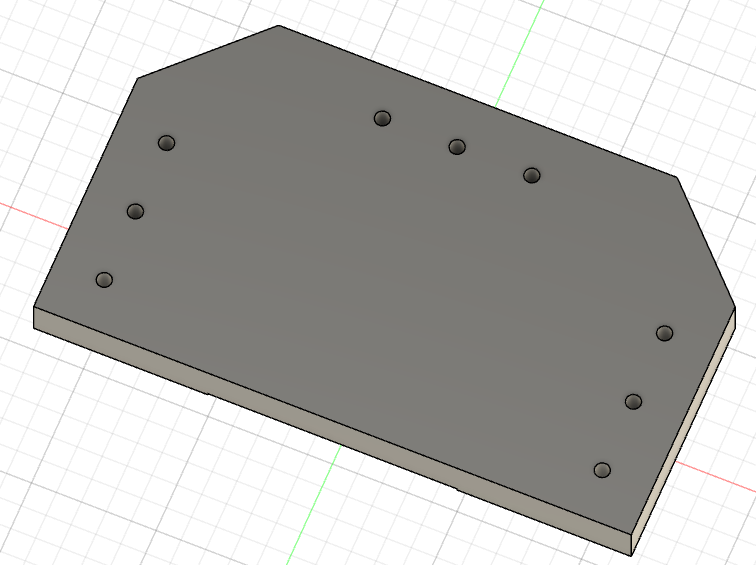
\includegraphics[width=\textwidth]{Main/Ch4/3D_models/clamp-top-top.png}
        \caption{Clamp front-section, groove for holding sample.}
    \end{subfigure}
    ~
    \begin{subfigure}[t]{0.5\textwidth}
        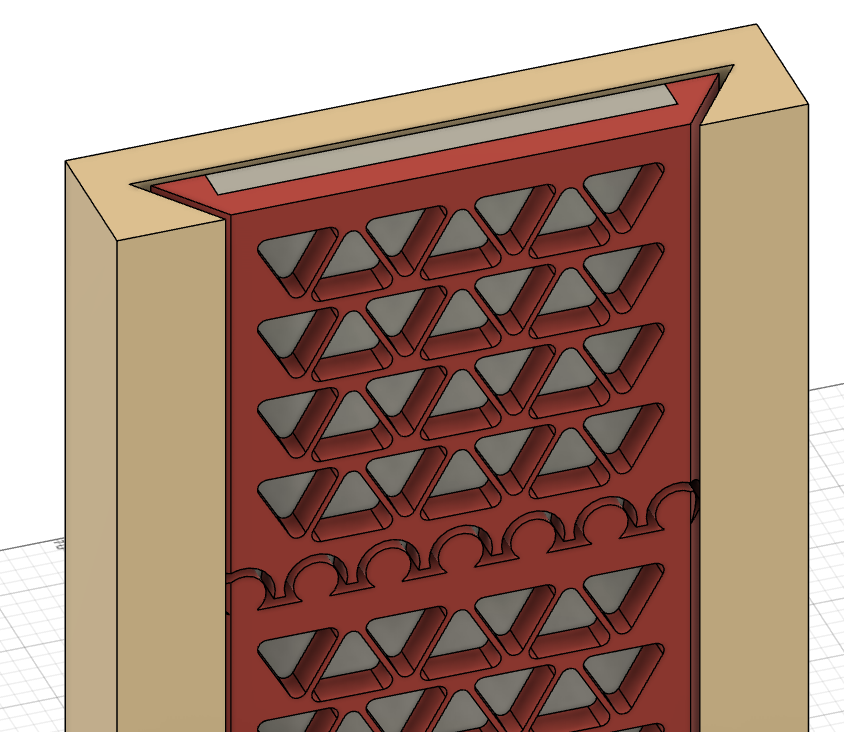
\includegraphics[width=\textwidth]{Main/Ch4/3D_models/Anode-Holder-Full-Assembly.png}
        \caption{Anode holder assembly (open-face facing cathode in red, closed-face facing beaker in tan, indium bar in grey).}
    \end{subfigure}
    ~
    \begin{subfigure}[t]{0.5\textwidth}
        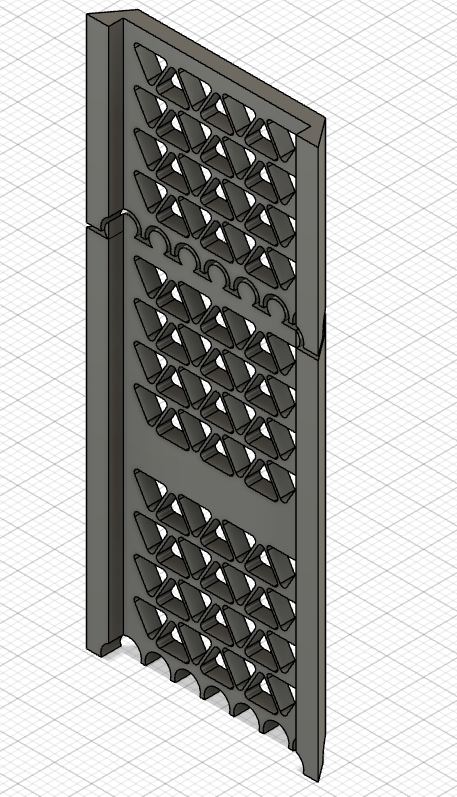
\includegraphics[width=\textwidth]{Main/Ch4/3D_models/Anode-Holder-Open-Face.png}
        \caption{Open face section of anode holder with slices for 3D printing or smaller CNC machines.}
    \end{subfigure}
    \caption{3D models of assemblies for improving electroplating setup}
    \label{fig:3D_models}
\end{figure}


Since the 3D designs in \ref{fig:3D_models} would meet the specifications indicated earlier, appropriate material selection would be required.

As such materials were selected to meet chemical resistance properties for the harshest chemicals that would be used in the process ($15\% \ch{HCl}$). While a variety of plastics met the requirements including PEEK, PTFE, HDPE and many others \cite{margolis2006engineering}, HDPE was selected as it was many orders of magnitude cheaper than PEEK or PTFE and was also much more easily machinable.

This selection would allow for more easy prototyping while meeting all the functional requirements.


